
\documentclass[10pt,a4paper]{article}
\usepackage[utf8]{inputenc}
\usepackage[spanish]{babel}
\usepackage{amsmath}
\usepackage{amsfonts}
\usepackage{amssymb}
\usepackage{makeidx}
\usepackage{graphicx}
\usepackage{cite} % para contraer referencias
\usepackage{fourier}
\usepackage{xcolor}
\usepackage{hyperref}
 \usepackage{float}
\usepackage[bottom]{footmisc}
\usepackage[left=2cm,right=2cm,top=2cm,bottom=2cm]{geometry}
\title{Plan - sesión 3}


\author{\textbf{Victor M. Santos}\thanks{victorhugo\_m09@hotmail.com}, \textbf{M.Tarazona-Alvarado}\thanks{miguelta281@gmail.com}, \textbf{J. Pisco-Guabave} \thanks{jhojavi@gmail.com}. \\ Grupo Halley , \\ Universidad Industrial de Santander, Bucaramanga, Colombia.}


\date{ }


\begin{document}

\maketitle
\tableofcontents
\section{Objetivo}
Comparar las distancias y tamaños de los cuerpos del Sistema Solar.

\section{Contenido}
\begin{itemize}
\item Unidades astronómicas
\item Distancias y tamaños en el Sistema Solar
\item Paralaje
\end{itemize}


\section{Recursos}
\begin{itemize}
 \item Salón con capacidad para 20 personas
 \item Proyector
 \item Computador
 \item Marcadores
 \item Tablero
 \item Espacio al aire libre (amplio)
\end{itemize}

\section{Marco conceptual}
El universo es vasto y desconocemos sus límites, si es que los tiene. Históricamente los científicos se han esforzado por desenmascarar las verdades ocultas en el cosmos, teorizando sobre la composición de todas las cosas que podemos sentir como la madera, el agua o el aire. Conforme la ciencia avanzaba, se descubrían nuevos límites, tanto en lo pequeño como en lo grande, desde los átomos hasta las galaxias. 

\subsection{Unidades astronómicas}
Las distancias entre planetas y objetos astronómicos son gigantescas si las comparamos con las distancias que medimos en la cotidianidad. Con el objetivo de usar una unidad conveniente para describir las distancias en el sistema solar, el mundo científico optó por definir la Unidad Astronómica (UA). Esta unidad se definió como la distancia media de la Tierra al Sol y es equivalente 149.597.870.700 metros.

\begin{figure}[H]
\centering
%\raggedright
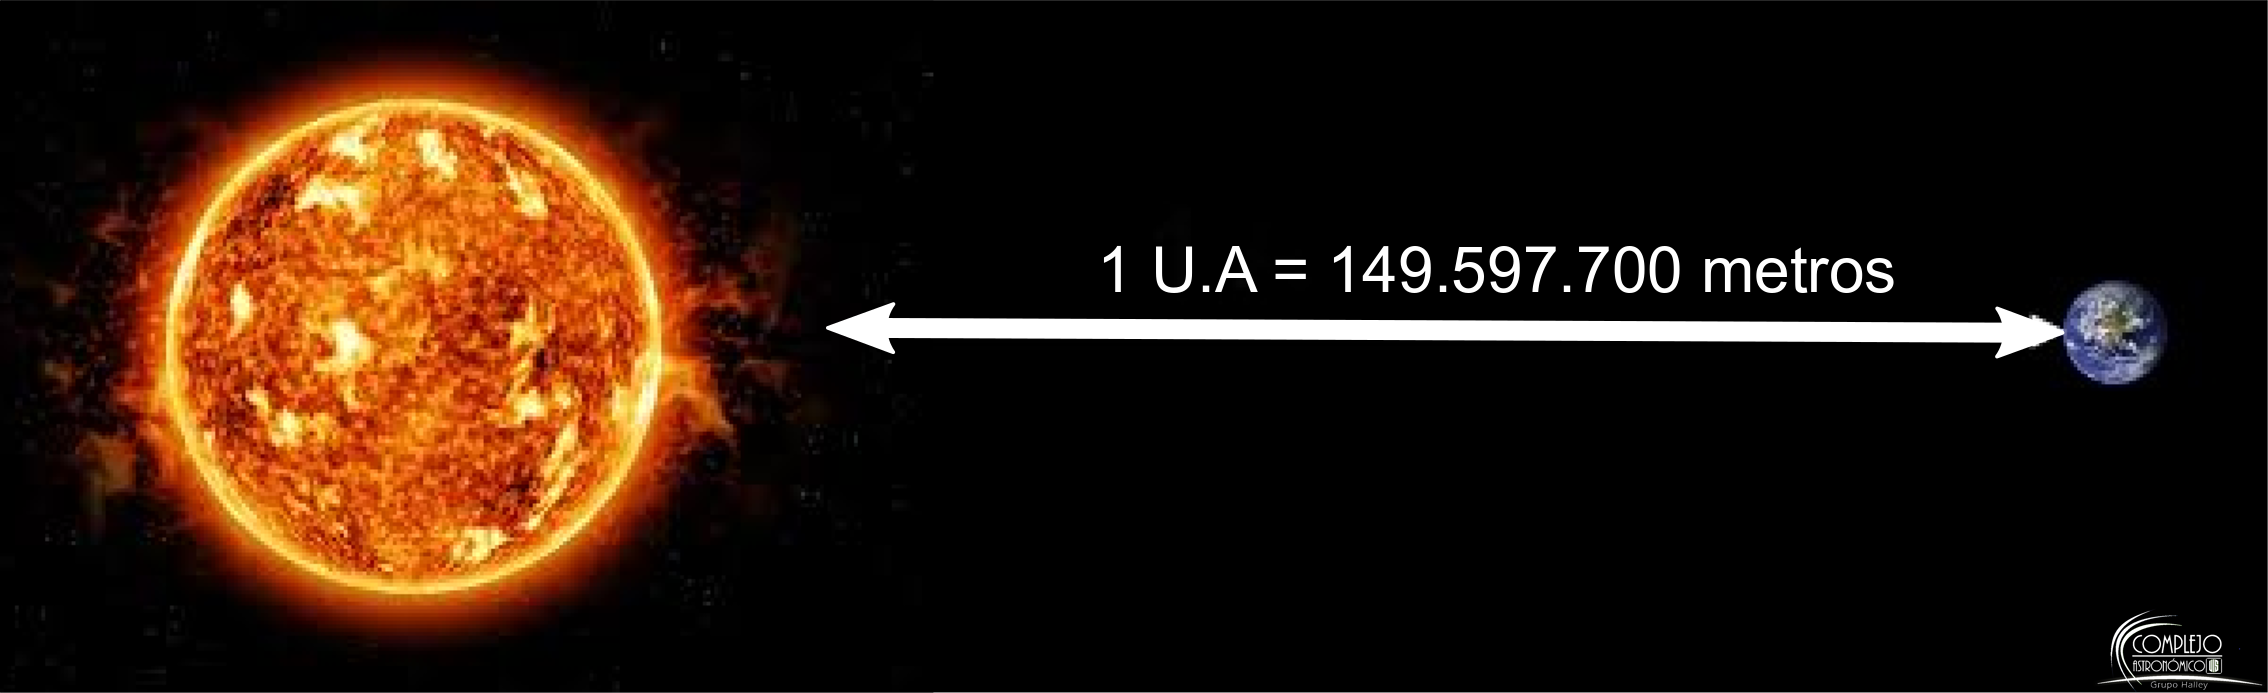
\includegraphics[scale=0.18]{Imagenes/Unidad_astro_01}
\end{figure}
  
  
\subsection{Distancias y tamaños en el Sistema Solar}
\begin{figure}[H]
\centering
%\raggedright
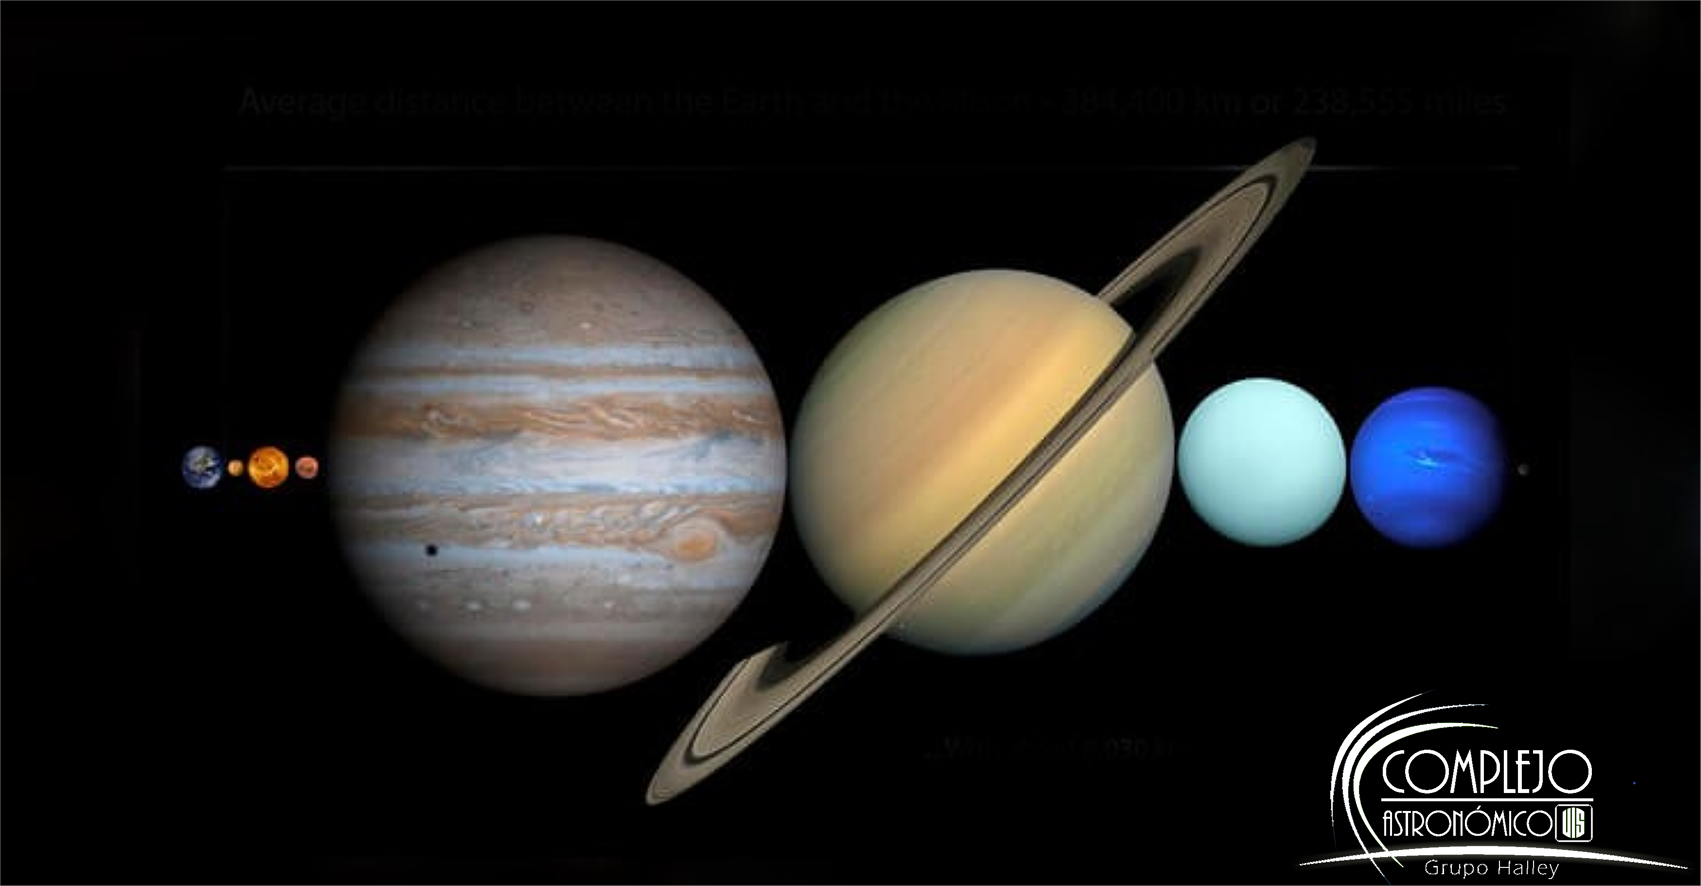
\includegraphics[scale=0.18]{Imagenes/Tamanos_01}
\end{figure}
Al hablar del Sistemas Solar los astrónomos se refieren a un espacio delimitado, con centro en el Sol y pasando por varios cuerpos planetarios hasta llegar a la nube de Oort. El Sol tiene la mayor parte de la masa del Sistema Solar, sumando las masas de todos los planetas y lunas solo se llega a 1/700 de la masa solar. Algunos datos del Sol son:

\begin{itemize}
\item \textbf{Radio:} $6.9635 \times 10^{10}$ [$cm$] $\rightarrow 109$ veces el terrestre.
\item \textbf{Superficie:} $6.0936 \times 10^{22}$ [$cm$] $\rightarrow 11880$ veces la terrestre.  
\item \textbf{Volumen:} $1.4144 \times 10^{33}$ [$cm^{3}$] $\rightarrow 1.306 \times 10^{6}$ veces el terrestre.
\item \textbf{Masa:} $1.993 \times 10^{33}$ [$g$] $\rightarrow 332.270$ veces la terrestre.
\item \textbf{Paralaje:} $8.79''$
\item \textbf{Tipo espectral:} $G2$
\item \textbf{Magnitud absoluta:} $+4.73$
\item \textbf{Magnitud aparente:} $-26.84$
\item \textbf{Distancia media Sol-Tierra:} $1.496 \times 10^{12}$ [$cm$]
\item \textbf{Distancia mínima (perihelio):} $1.4688 \times 10^{13}$ [$cm$]
\item \textbf{Distancia máxima (afelio):} $1.5189 \times 10^{13}$ [$cm$]
\end{itemize}

En cuanto a los planetas, la Unión Astronómica Internacional (IAU) los definió como cuerpos celestes que están en órbita alrededor del Sol, con forma esférica y que su órbita esté despejada de otros cuerpos. En cambio, un planeta enano es un cuerpo que también está en órbita alrededor del Sol y también es redondo, pero no que no ha despejado su órbita y que no es un satélite.

\begin{table}[h]
\begin{tabular}{|l|c|c|c|c|c|c|c|c|}
\hline
                                                                                                       & \textbf{Mercurio} & \textbf{Venus} & \textbf{Tierra} & \textbf{Marte} & \textbf{Jupiter} & \textbf{Saturno} & \textbf{Urano} & \textbf{Neptuno} \\ \hline
\multicolumn{1}{|c|}{\textbf{\begin{tabular}[c]{@{}c@{}}Distancia media del \\ Sol U.A.\end{tabular}}} & 0.387             & 0.723          & 1               & 1.524          & 5.203            & 9.539            & 19.18          & 30.06            \\ \hline
\textbf{\begin{tabular}[c]{@{}l@{}}Inclinación de la órbita \\ respecto a la eclíptica\end{tabular}}   & 7°                & 3°,4           & 0°              & 1°,9           & 1°,3             & 2°,5             & 0,8°           & 1.8°             \\ \hline
\textbf{Radio en el ecuador {[}km{]}}                                                                  & 2489              & 6310           & 6378            & 3389,9         & 71714            & 60330            & 26200          & 25225            \\ \hline
\textbf{Masa (Tierra = 1)}                                                                             & 0,055             & 0,815          & 1               & 0,108          & 318,1            & 95,147           & 14,6           & 17,2             \\ \hline
\end{tabular}
\end{table}


\subsection{Paralaje}
El paralaje es un término cuyo significado se remonta a la Grecia antigua. Este concepto deriva de la concepción de cambio y se relaciona estrechamente con los movimientos de los astros. En astronomía, el paralaje es el ángulo formado por la dirección de dos líneas visuales relativas a la observación de un mismo astro desde dos puntos distintos.

\begin{figure}[H]
\centering
%\raggedright
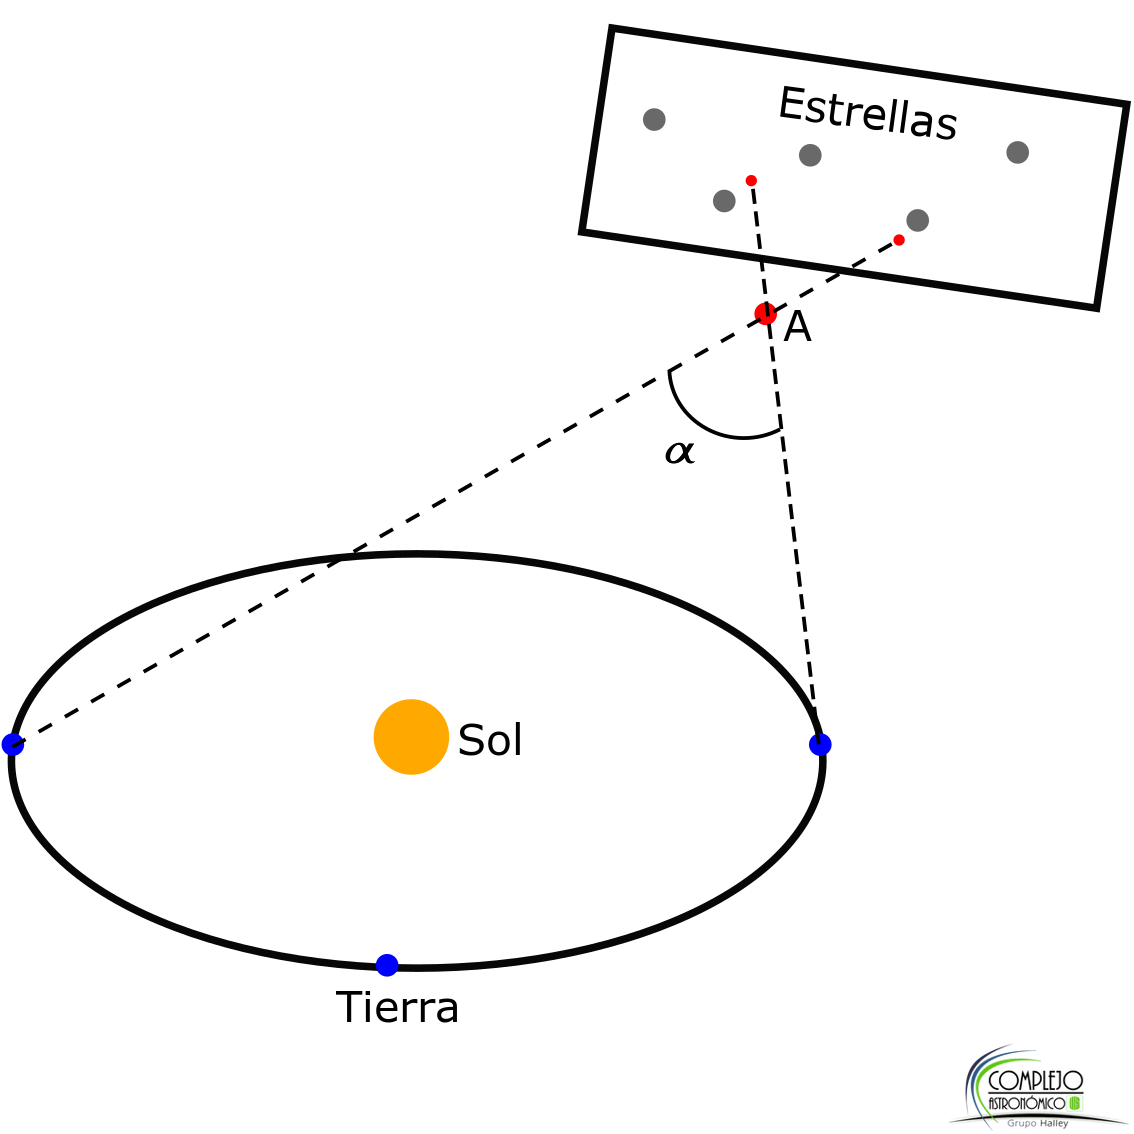
\includegraphics[scale=0.18]{Imagenes/Paralaje_01}
\end{figure}


\section{Planeación de la sesión}
\begin{table}[H]
\begin{tabular}{|l|l|l|l|}
\hline
\textbf{Etapa}      & \textbf{Tiempo} & \textbf{Actividad}                                        & \textbf{Recursos}                                                           \\ \hline
\textbf{Inicio}     & 20 minutos      & \begin{tabular}[c]{@{}l@{}}S03AI01 \\S03AI02   \end{tabular}                                                  & \begin{tabular}[c]{@{}l@{}}- Cuerda \\ - Compás  \\ -Tijeras \\ - Cartulina (cartón paja)  \end{tabular} \\ \hline
\textbf{Desarrollo} &   50 minutos               & S03AD01  & \begin{tabular}[c]{@{}l@{}}- Cuerda \\ - Compás  \\ -Tijeras \\ - Cartulina (cartón paja) \\ - Metro (regla)\\
 \end{tabular}         \\ \hline
\textbf{Cierre}     &   50 minutos              &  \begin{tabular}[c]{@{}l@{}}S03AC01   \\S03AC01    \end{tabular}                                                                                           & \begin{tabular}[c]{@{}l@{}} - Medidor de paralaje \\ - Metro  \end{tabular} \\ \hline
\end{tabular}
\end{table}

\subsection{S03AI01}
Para esta actividad, 9 estudiantes serán ubicados por un compañero con la intención de representar las distancias entre el Sol y los planetas del Sistema Solar. Los estudiantes realizarán la actividad con base en sus creencias y conocimientos previos, sin correcciones del docente o del tutor. Los estudiantes se valdrán de una cuerda de tamaño (4,5 [m]) que representa la distancia del Sol a Neptuno para ubicarse.

\begin{table}[H]
\begin{tabular}{|c|c|c|}
\hline
\textbf{Objeto}   & \textbf{Distancia al Sol{[}km{]}}                                      & \textbf{Distancia al Sol  {[}cm{]}} \\ \hline
\textbf{Mercurio} &  57.910.000    & 5.791                   \\ \hline
\textbf{Venus}    & 108.200.000   & 10.82                   \\ \hline
\textbf{Tierra}   & 146.600.000  & 14.66                   \\ \hline
\textbf{Marte}    & 227.940.000    & 22.794                  \\ \hline
\textbf{Júpiter}  & 778.330.000   & 77.833                  \\ \hline
\textbf{Saturno}  & 1.429.400.000 & 142.94                  \\ \hline
\textbf{Urano}    & 2.870.990.000   & 287.099                 \\ \hline
\textbf{Neptuno}  & 4.504.300.000     & 450.43                  \\ \hline
\end{tabular}
\end{table}

\subsection{S03AI02}
Para esta actividad, se repartirá una figura correspondiente a un planeta a cada estudiantes (estas figuras deben estar listas antes de la clase y serán de los planetas a tamaño a escala). Cada estudiante debe identificar cuál planeta tiene y organizarlos según su distancia al Sol. \\

\begin{table}[H]
\begin{tabular}{|c|c|c|}
\hline
\textbf{Objeto}   & \textbf{Radio {[}km{]}}                               & \textbf{Radio {[}cm{]}} \\ \hline
\textbf{Sol}      & 696.340                                               & 139.268                 \\ \hline
\textbf{Mercurio} &  2.44  & 0.48                    \\ \hline
\textbf{Venus}    & 6.052  & 1.21           \\ \hline
\textbf{Tierra}   & 6.378                                                 & 1.28                    \\ \hline
\textbf{Marte}    & 3.397   & 0.68                    \\ \hline
\textbf{Júpiter}  &  71.492 & 14.30            \\ \hline
\textbf{Saturno}  &60.268 & 12.05       \\ \hline
\textbf{Urano}    & 25.559                                                & 5.11                    \\ \hline
\textbf{Neptuno}  & 24.746                                                & 4.94                    \\ \hline
\end{tabular}
\end{table}

\subsection{S03AD01}
Esta actividad es una charla que se vale de diferentes maquetas para enseñar los contenidos. Al introducir los temas de tamaños y distancias, el tutor deberá explicar el concepto de Unidad Astronómica acompañado de la imagen en la presentación. Luego, deberá presentar una pregunta problema del tipo: "Si el planeta Tierra fuera del tamaño de una pelota de basquetball, entonces ¿a qué distancia está la Luna de él?". A continuación, se muestra que siguiendo esa escala, la Luna sería del tamaño de una pelota de tenis, y además estaría una distancia tan grande que la pelota de basketball (la Tierra) cabría 30 veces entre las dos pelotas. \\

Habiendo culminado con la representación anterior, se muestra una cuerda que representa la distancia del Sol a Neptuno (la misma usada en la actividad de inicio) para ubicar correctamente los planetas del Sistema Solar. Luego, tomando como base la actividad de tamaños inicial, se comparará lo hecho por los estudiantes con los radios reales y a escala de cada uno de los planetas. Para concluir, se explica (con ayuda de la presentación) la actividad de cierre con el medidor de paralaje.

\subsection{S03AC01}
Para esta actividad haremos uso del Medidor de Paralaje. El primer ejercicio (\textbf{Imagen \ref{paralaje_2}}) consiste en ubicar el medidor y un objeto en el suelo y de frente. Luego, se desplaza el medidor de paralaje a 10 metros de la distancia inicial. A continuación se aleja el objeto, de forma perpendicular al medidor, con una variación de 50 centímetros hasta los 200 centímetros. En cada punto (1, 2, 3 y 4) se toma la medida del ángulo y luego se contrasta con el desplazamiento del medidor de paralaje.

\begin{figure}[H]
\centering
%\raggedright
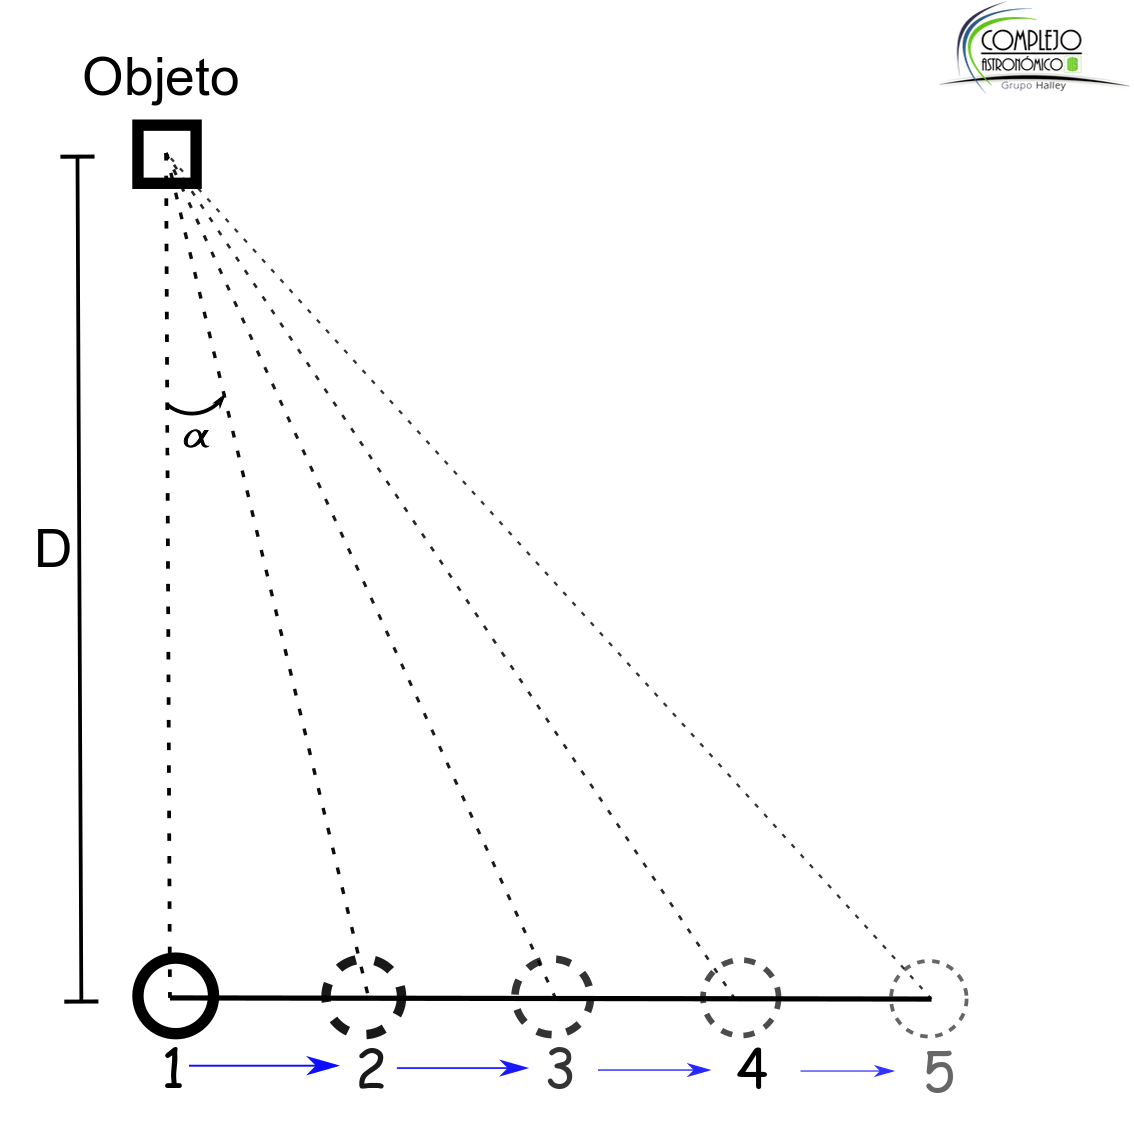
\includegraphics[scale=0.18]{Imagenes/Paralaje_02}
\caption{Ejercicio 1}
\label{paralaje_2}
\end{figure}

\subsection{S03AC02}
Para esta actividad haremos uso del Medidor de Paralaje. El este ejercicio consiste  en ubicar el medidor y un objeto en el suelo y de frente. Luego, se desplaza el medidor de paralaje a 10 metros de distancia de la posición inicial. A continuación se aleja el objeto, de forma perpendicular al medidor, con una variación de 50 centímetros hasta los 10 centímetros, como se muestra en la figura (\ref{paralaje_3}) se toma la medida del ángulo y luego se contrasta con el desplazamiento del objeto.
\begin{figure}[H]
\centering
%\raggedright
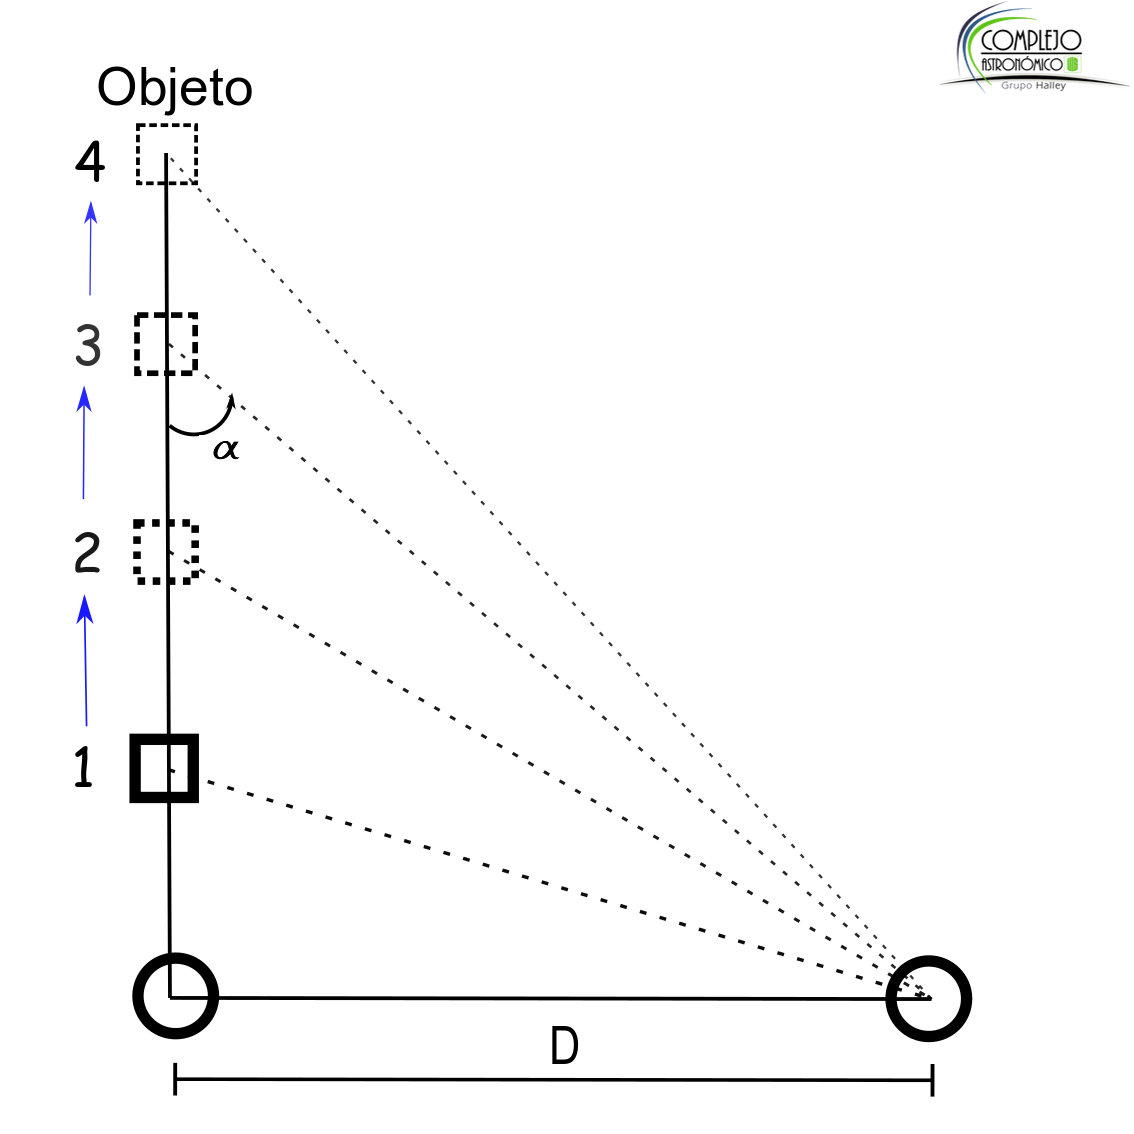
\includegraphics[scale=0.18]{Imagenes/Paralaje_03}
\caption{Ejercicio 2}
\label{paralaje_3}
\end{figure}
\end{document}